\documentclass[
	letterpaper, % Paper size, specify a4paper (A4) or letterpaper (US letter)
	10pt, % Default font size, specify 10pt, 11pt or 12pt
]{CSUniSchoolLabReport}

%----------------------------------------------------------------------------------------
%	REPORT INFORMATION
%----------------------------------------------------------------------------------------

\title{Spice \& Circuits \\ Circuits \& Signals \\ EECE2150} % Report title

\author{Michael \textsc{Brodskiy}}

\date{January 26, 2023} % Date of the report

%----------------------------------------------------------------------------------------


\begin{document}

\maketitle % Insert the title, author and date using the information specified above

\begin{center}
	\begin{tabular}{l r}
		Date Performed: & January 19, 2023 \\ % Date the experiment was performed
        Partner: & Juan \textsc{Zapata} \\ % Partner names
		Instructor: & Professor \textsc{Sun} % Instructor/supervisor
	\end{tabular}
\end{center}

\setcounter{section}{-1}

\section{Introduction}

The purpose of this laboratory experimentation is two-fold: firstly, to allow us to orient ourselves with the practice of circuit modeling through Spice; and secondly, to allow an introduction of AC current and its behavior in circuitry

\section{Spice Modeling}

\subsection{Q1} PSpice indicates the direction of the current by applying a sign to it in the NetList

\subsection{Q2} The currents at each node do add to zero as expected. This results in the following (in milliamperes):

\begin{equation}
  2.30769 - 1.53846 - .759231 \approx 0 [\si{\ampere}]
  \label{eq:1}
\end{equation}

\subsection{Q3} The voltages around each of the loops also add to zero as expected. They result in the following:

\begin{equation}
  \begin{split}
    10 - 2.30769 - 7.69231 &= 0[\si{\volt}]\\ 
    10 - 4.61538 - 5.385 &= 0[\si{\volt}]
\end{split}
  \label{eq:2}
\end{equation}

\subsection{Q4} The best way to keep track of the voltages is to trace the path from the ground node to another node, and keeping any subsequent signage consistent with the first one (whether using positive or negative).

\section{AC Circuits}

\begin{figure}[h!]
  \centering
  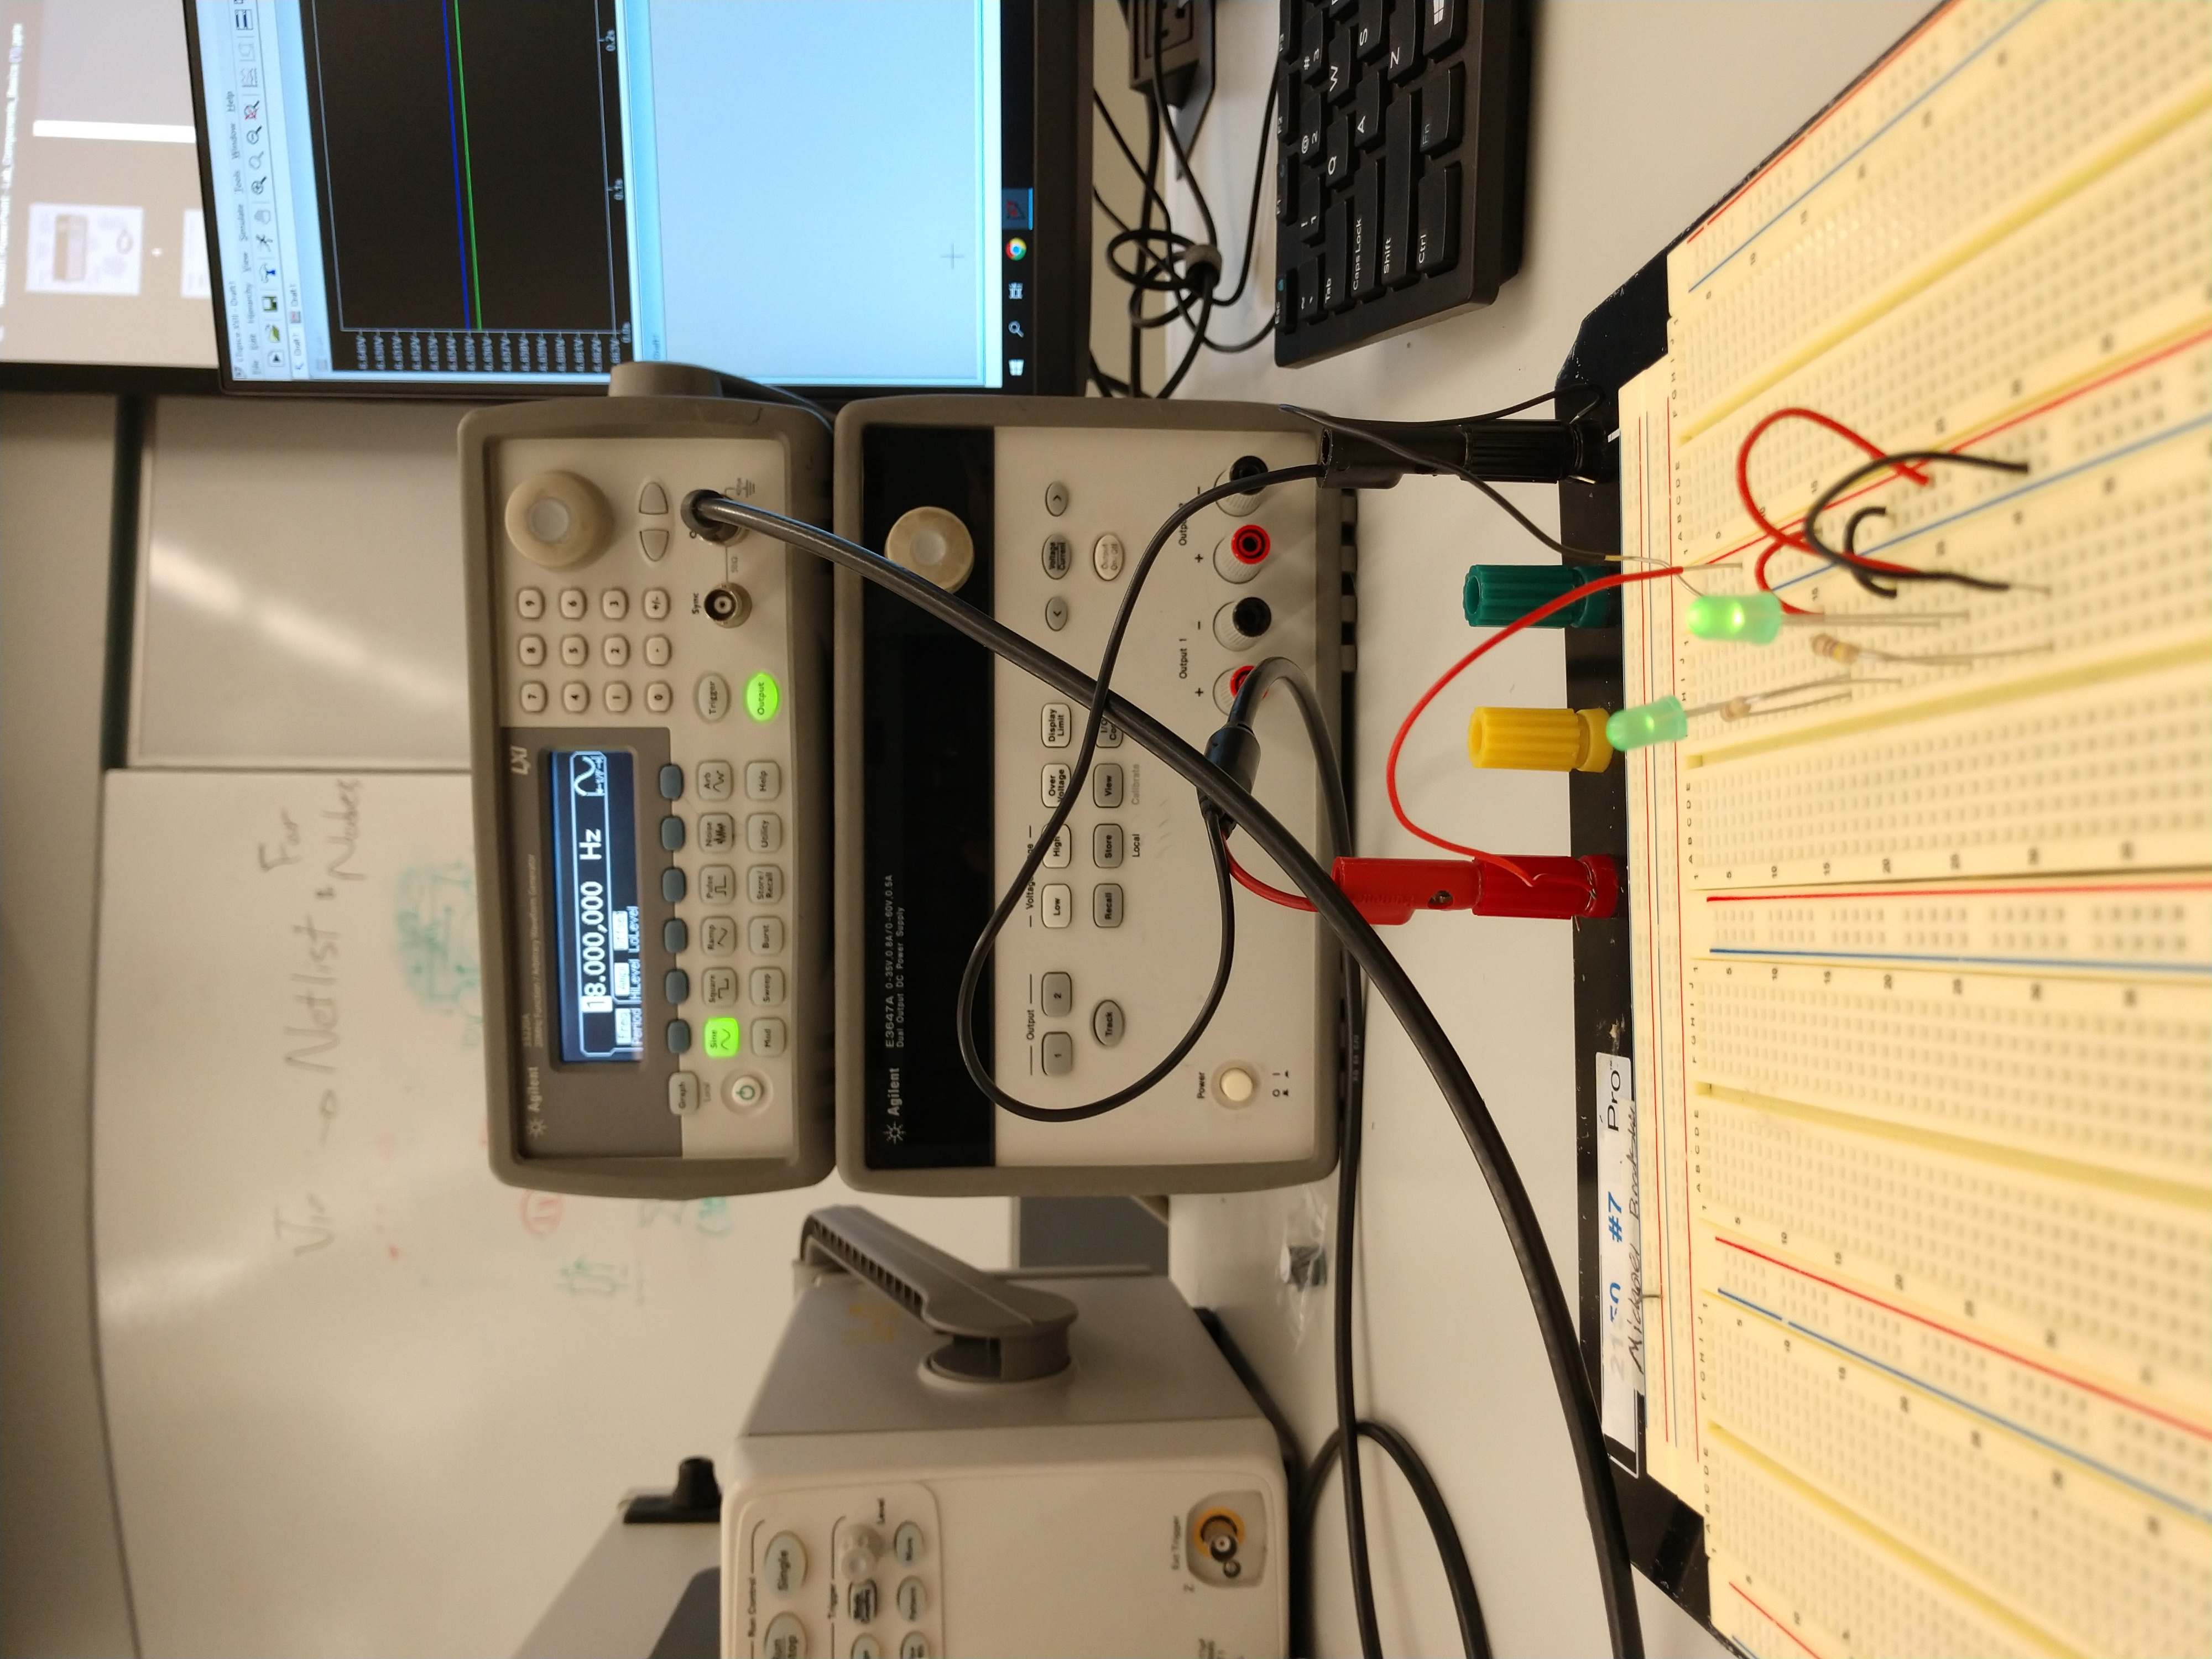
\includegraphics[width=.9\textwidth, angle=270]{Figures/L3C1.jpg}
  \caption{The Constructed LED Circuit}
  \label{fig:1}
\end{figure}

\subsection{Q5} The two LEDs should \underline{never} blink at the same time (though, at some point, it may seem like it to the human eye). This is because AC current functions by oscillating from positive to negative values; due to the configuration in this section, the AC current is fluctuating as a square wave, which means either one light or the other is on, as the diodes have opposing polarities and are switched, while the voltage is $\pm5[\si{\volt}]$.

\subsection{Triangle and Sine Waves} When setting the wave type to triangle, one LED fades in fully, then shuts off, while the other switches on fully, and then fades out. This pattern is then repeated. For sine waves, one fades in while the other is off, and vice versa.

\subsection{Q6} The blinking stops at slightly above the frequency of $40[\si{\hertz}]$. This value remains the same whether it is triangle, sine, or square; however, depending on some peoples' vision, it could be slightly different for them (albeit not by much). The light intensity probably has little effect, but if the experiment were performed in a darker room, it would probably be easier to see. Using a camera to record the blinking allows it to be seen at this frequency, so the limiting factor is most likely human vision.

\subsection{Q7} It is quite different to be able to even slightly tell that the two are out of phase (via human eye, camera recordings make it easier), the frequency needs to be below $15[\si{\hertz}]$. Even then, it is difficult to tell, and, as such, would be better if lowered further.

\section{Conclusion}

Modeling a simple circuit, whose true values were simply calculable by hand allowed for an adequate introduction to Spice circuit modeling. Additionally, the application of a function generator, in tandem with an oscilloscope and constructed circuit allowed for a simple introduction of alternating current.

\end{document}
